% --- CHUNK_METADATA_START ---
% src_checksum: fc3384bbcbb9eae9657d8b4e77a05ea21d8f91414f3c33fd9d7201ca00922c09
% needs_review: True
% --- CHUNK_METADATA_END ---
\chapter{Infinite sequences of random variables}% --- CHUNK_METADATA_START ---
% src_checksum: 2a7f2c7c7174c665a05520a7d0b71d6166affe8b95f8a267ffb2fdec322379cd
% needs_review: True
% --- CHUNK_METADATA_END ---
\sloppy
Let $(\Omega, \mathcal{F}, P)$ be a probability space.% --- CHUNK_METADATA_START ---
% src_checksum: 62a672d4b2b4d6d9960ce59ec881538446140e9c93a7045c3d3824e8580c7a2d
% needs_review: True
% --- CHUNK_METADATA_END ---
\section{Convergence modes}% --- CHUNK_METADATA_START ---
% src_checksum: 25e80a25b38330a3945183430f8398a3d79b38e313d2e6bd0aec108003aaa213
% needs_review: True
% --- CHUNK_METADATA_END ---
Let $(X_n)_{n \in \mathbb{N}}$ be a sequence of random variables (r.v.) defined on $(\Omega, \mathcal{F}, P)$. Let also $X$ be another r.v. defined on $(\Omega, \mathcal{F}, P)$.% --- CHUNK_METADATA_START ---
% src_checksum: 799df6a6f0d4480427572c06e0358a239097f3dda8db9d2629629f933cf5a2f2
% needs_review: True
% --- CHUNK_METADATA_END ---

\begin{definition}[Almost Sure Convergence]
The sequence $(X_n)_{n \in \mathbb{N}}$ converges almost surely to $X$, which we denote by $X_n \xrightarrow{p.s.} X$, if
\[
P(\{\omega \in \Omega : \lim_{n \to \infty} X_n(\omega) = X(\omega)\}) = 1.
\]
\end{definition}
% --- CHUNK_METADATA_START ---
% src_checksum: 728b857b511b7f51c8cb0de12513571ff7580205e43e24086bc89193ce248b44
% needs_review: True
% --- CHUNK_METADATA_END ---
\begin{definition}[Convergence in Mean of Order $r$ ($L^r$)]
Let $r \geq 1$. The sequence $(X_n)_{n \in \mathbb{N}}$ converges to $X$ in $L^r(\Omega, P)$, denoted by $X_n \xrightarrow{L^r} X$, if
\[
\lim_{n \to \infty} \mathbb{E}[|X_n - X|^r] = 0.
\]
\end{definition}% --- CHUNK_METADATA_START ---
% src_checksum: eac08c4171c4c910e485d0edbbaa4fe0e1d6ddb601b057533972b0dc1410dd90
% needs_review: True
% --- CHUNK_METADATA_END ---
\begin{definition}[Convergence in Probability]
The sequence $(X_n)_{n \in \mathbb{N}}$ converges to $X$ in probability, denoted as $X_n \xrightarrow{P} X$, if
\[
\forall \varepsilon > 0, \quad \lim_{n \to \infty} P(|X_n - X| > \varepsilon) = 0.
\]
\end{definition}% --- CHUNK_METADATA_START ---
% src_checksum: 701f5f66f39689b0d605faa2a781d005e86b4e86a02eef029759549fc41889fc
% needs_review: True
% --- CHUNK_METADATA_END ---
\section{Links between convergences}% --- CHUNK_METADATA_START ---
% src_checksum: 3f035032c64fc780ad39c4a784803d79cdcd5c6e12d69e6da2c1c2c27affdec2
% needs_review: True
% --- CHUNK_METADATA_END ---
The most difficult convergence to establish is almost sure convergence.% --- CHUNK_METADATA_START ---
% src_checksum: d54ad21950837960d6ae33db070349d806ad1a4ec0818fd9fa439a30916f9739
% needs_review: True
% --- CHUNK_METADATA_END ---
\begin{proposition}
If $X_n \xrightarrow{p.s.} X$, then $X_n \xrightarrow{P} X$.
\end{proposition}% --- CHUNK_METADATA_START ---
% src_checksum: dbcb68a542fd99a89311877c0be4dd31d6f1b6f5ef0d5eb2b37c1a6c6df13bbc
% needs_review: True
% --- CHUNK_METADATA_END ---

\begin{proof}
Assume $X_n \xrightarrow{p.s.} X$. By definition, this means that $P(\{\omega \in \Omega : \lim_{n \to \infty} X_n(\omega) = X(\omega)\}) = 1$.
The definition of the limit of a sequence is:
\[
\lim_{n \to \infty} X_n(\omega) = X(\omega) \iff \forall \varepsilon > 0, \exists N \in \mathbb{N}, \forall n > N, |X_n(\omega) - X(\omega)| < \varepsilon.
\]
For measurability reasons, we restrict $\varepsilon$ to positive rationals, which is sufficient.
\begin{align*}
    P(\lim_{n \to \infty} X_n = X) = 1 &\iff P\left(\forall \varepsilon \in \mathbb{Q}_+^*, \exists N \in \mathbb{N}, \forall n > N, |X_n - X| < \varepsilon\right) = 1 \\
    &\iff P\left(\bigcap_{\varepsilon \in \mathbb{Q}_+^*} \bigcup_{N \in \mathbb{N}} \bigcap_{n > N} \{|X_n - X| < \varepsilon\}\right) = 1
\end{align*}
Since this is a countable intersection of events with probability 1, each of these events must have a probability of 1.
\[
\implies \forall \varepsilon > 0, \quad P\left(\bigcup_{N \in \mathbb{N}} \bigcap_{n > N} \{|X_n - X| < \varepsilon\}\right) = 1
\]
Taking the complement, the probability becomes 0:
\[
\forall \varepsilon > 0, \quad P\left(\left(\bigcup_{N \in \mathbb{N}} \bigcap_{n > N} \{|X_n - X| < \varepsilon\}\right)^c\right) = P\left(\bigcap_{N \in \mathbb{N}} \bigcup_{n > N} \{|X_n - X| \geq \varepsilon\}\right) = 0
\]
Let $A_N = \bigcup_{n > N} \{|X_n - X| \geq \varepsilon\}$. The sequence of events $(A_N)_{N \in \mathbb{N}}$ is decreasing. By continuity of the probability measure for decreasing sequences, we have:
\[
P\left(\bigcap_{N \in \mathbb{N}} A_N\right) = \lim_{N \to \infty} P(A_N) = \lim_{N \to \infty} P\left(\bigcup_{n > N} \{|X_n - X| \geq \varepsilon\}\right) = 0.
\]
However, for all $N$, we have the inclusion $\{|X_N - X| \geq \varepsilon\} \subset \bigcup_{n > N} \{|X_n - X| \geq \varepsilon\}$.
Therefore, $P(|X_N - X| \geq \varepsilon) \leq P(\bigcup_{n > N} \{|X_n - X| \geq \varepsilon\})$. Taking the limit as $N \to \infty$, we obtain:
\[
\forall \varepsilon > 0, \quad \lim_{N \to \infty} P(|X_N - X| \geq \varepsilon) = 0.
\]
This is the definition of convergence in probability, $X_n \xrightarrow{P} X$.
\end{proof}
% --- CHUNK_METADATA_START ---
% src_checksum: 78424311d1fe1df7fd1c846fdad282aaabbc8f03095274ab41b9111953cb9e63
% needs_review: True
% --- CHUNK_METADATA_END ---

\begin{proposition}
Let $r \geq 1$. If $X_n \xrightarrow{L^r} X$, then $X_n \xrightarrow{P} X$.
\end{proposition}
% --- CHUNK_METADATA_START ---
% src_checksum: b9dd64c527eb156fd27c1efef66af80eff88f48209ff81c377df351a33b475fd
% needs_review: True
% --- CHUNK_METADATA_END ---
\begin{proof}
Let $\varepsilon > 0$. We use Markov's inequality. Let's write:
\begin{align*}
    \mathbb{E}[|X_n - X|^r] &= \int_{\Omega} |X_n - X|^r dP \\
    &= \int_{\{|X_n - X| \geq \varepsilon\}} |X_n - X|^r dP + \int_{\{|X_n - X| < \varepsilon\}} |X_n - X|^r dP \\
    &\geq \int_{\{|X_n - X| \geq \varepsilon\}} |X_n - X|^r dP \\
    &\geq \int_{\{|X_n - X| \geq \varepsilon\}} \varepsilon^r dP = \varepsilon^r P(|X_n - X| \geq \varepsilon).
\end{align*}
From this, we obtain:
\[
P(|X_n - X| > \varepsilon) \leq \frac{1}{\varepsilon^r} \mathbb{E}[|X_n - X|^r].
\]
Since $X_n \xrightarrow{L^r} X$, we have $\lim_{n \to \infty} \mathbb{E}[|X_n - X|^r] = 0$. Therefore,
\[
\lim_{n \to \infty} P(|X_n - X| > \varepsilon) = 0,
\]
which proves that $X_n \xrightarrow{P} X$.
\end{proof}% --- CHUNK_METADATA_START ---
% src_checksum: 2b4abd574a7e1454560748697304735834230b020a578c46375cddbbe84b24e2
% needs_review: True
% --- CHUNK_METADATA_END ---
\begin{proposition}[Compatibility with Addition]
If $X_n \xrightarrow{*} X$ and $Y_n \xrightarrow{*} Y$, then $X_n + Y_n \xrightarrow{*} X+Y$, where $*$ can be almost sure convergence, $L^r$ (with the same $r \ge 1$), or convergence in probability.
\end{proposition}% --- CHUNK_METADATA_START ---
% src_checksum: 8feb7731b1c2962ce7a1443d5273827bdd1b324187d890ac35e586f9a8ed6a70
% needs_review: True
% --- CHUNK_METADATA_END ---
\begin{proof}[Hint for Convergence in Probability]
We use the triangle inequality and the sub-additivity of probability. For all $\varepsilon > 0$:
\[
\{|(X_n+Y_n) - (X+Y)| > \varepsilon\} \subset \{|X_n-X| + |Y_n-Y| > \varepsilon\} \subset \{|X_n-X| > \varepsilon/2\} \cup \{|Y_n-Y| > \varepsilon/2\}.
\]
Hence,
\[
P(|(X_n+Y_n) - (X+Y)| > \varepsilon) \leq P(|X_n-X| > \varepsilon/2) + P(|Y_n-Y| > \varepsilon/2).
\]
Each of the terms on the right tends to 0 as $n \to \infty$.
\end{proof}% --- CHUNK_METADATA_START ---
% src_checksum: 4cf36b51fc3b7417474242d80ffef9a4e1200a27060b60d86a2ab49ae379ca34
% needs_review: True
% --- CHUNK_METADATA_END ---
We can also translate classical measure theory theorems into the language of random variables.% --- CHUNK_METADATA_START ---
% src_checksum: 03cacfd671869f6194aa5176930c97f1085d28c9be183b63c2efac4413a0cba9
% needs_review: True
% --- CHUNK_METADATA_END ---
\begin{example}[Dominated Convergence Theorem]
Let $(X_n)$ be a sequence of random variables such that:
\begin{enumerate}
    \item There exists a random variable $X$ such that $X_n \xrightarrow{p.s.} X$.
    \item There exists a random variable $Y \geq 0$ that is integrable ($\mathbb{E}[Y] < \infty$) such that $|X_n| \leq Y$ almost surely for all $n$.
\end{enumerate}
Then $X_n \xrightarrow{L^1} X$, and in particular, $\lim_{n \to \infty} \mathbb{E}[X_n] = \mathbb{E}[X]$.
\end{example}% --- CHUNK_METADATA_START ---
% src_checksum: 4c2b0cf6ab193be1edbe20a8f9a5316bfb9292f6f34bdb1096789b56f7372621
% needs_review: True
% --- CHUNK_METADATA_END ---
\section{Examples}% --- CHUNK_METADATA_START ---
% src_checksum: 40c9b3b4952c4038b68ff4d675c5c90726fcad95a79ebf8050cf37ff49acfe03
% needs_review: True
% --- CHUNK_METADATA_END ---
We consider the probability space $(\Omega, \mathcal{F}, P) = ([0,1], \mathcal{B}([0,1]), \lambda_{|[0,1]})$, where $\lambda$ is the Lebesgue measure.% --- CHUNK_METADATA_START ---
% src_checksum: d1bb887cab6c11496eb40ba6f66323cd654a5e2e62f93f849e6e3bd4f3472498
% needs_review: True
% --- CHUNK_METADATA_END ---
\begin{example}
Consider the sequence of functions defined by $X_{2k}(\omega) = \mathbf{1}_{[0, 1/2]}(\omega)$ and $X_{2k+1}(\omega) = \mathbf{1}_{[1/2, 1]}(\omega)$ for $k \in \mathbb{N}$.
For any $\omega \in [0,1]$, the sequence $(X_n(\omega))$ oscillates between 0 and 1 (except at $\omega=1/2$) and thus does not converge. This sequence does not converge in any sense (a.s., $L^r$, or P).
\begin{figure}[H]
\centering
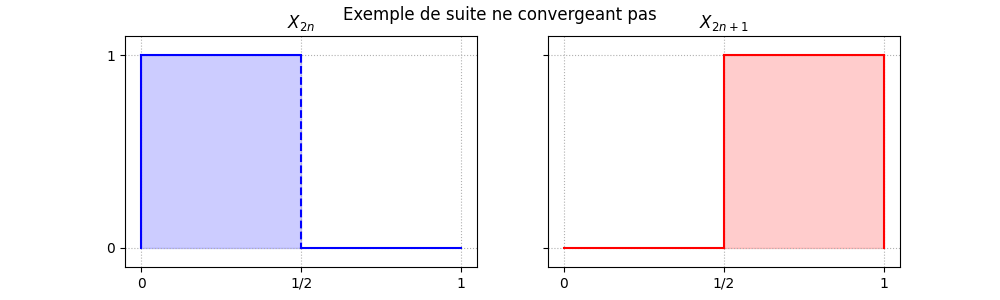
\includegraphics[width=0.7\textwidth]{ex3_plot1.png}
\caption{Sequence $(X_n)$ that has no limit.}
\label{fig:ex1_noconv}
\end{figure}
\end{example}% --- CHUNK_METADATA_START ---
% src_checksum: f78407ce50ed640c247bd16c10aed88d10bc614c6070d77f03c7e002db63a9fb
% needs_review: True
% --- CHUNK_METADATA_END ---
\begin{example}[The "Typewriter" Sequence]
Consider the sequence of random variables $(X_n)$ which are indicators of intervals that sweep $[0,1]$ with a width that tends to 0. For example:
$X_1 = \mathbf{1}_{[0,1]}$, $X_2 = \mathbf{1}_{[0,1/2]}$, $X_3 = \mathbf{1}_{[1/2,1]}$, $X_4 = \mathbf{1}_{[0,1/3]}$, etc.
This sequence converges in probability to 0, as the measure (length) of the interval where $X_n=1$ tends to 0.
\[
P(|X_n - 0| > \varepsilon) = P(X_n=1) \to 0 \quad \text{pour } 0 < \varepsilon < 1.
\]
However, for every $\omega \in [0,1]$, the sequence $X_n(\omega)$ takes the value 1 infinitely many times. Therefore, $\limsup_{n \to \infty} X_n(\omega) = 1$, while $\liminf_{n \to \infty} X_n(\omega) = 0$. The pointwise limit does not exist, so the sequence does not converge almost surely.
We thus have $X_n \xrightarrow{P} 0$ but $X_n \not\xrightarrow{p.s.} 0$.
\begin{figure}[H]
\centering
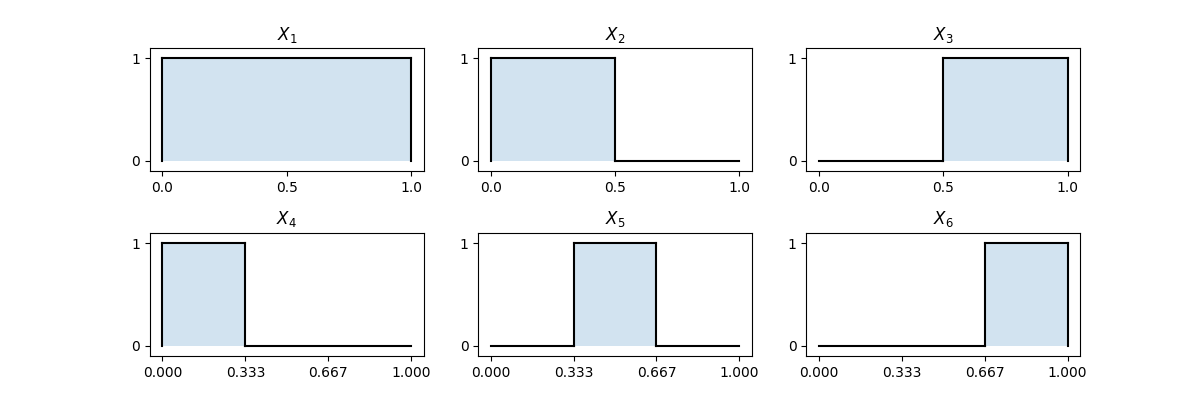
\includegraphics[width=\textwidth]{ex3_plot2.png}
\caption{The first terms of the "typewriter" sequence.}
\label{fig:typewriter}
\end{figure}
\end{example}% --- CHUNK_METADATA_START ---
% src_checksum: cbb99af2eea16f1b8ad102d9f2fa3887b268949834d28edfe207475ed32876e7
% needs_review: True
% --- CHUNK_METADATA_END ---
\section{Independence for an infinite sequence}% --- CHUNK_METADATA_START ---
% src_checksum: 25c325854c75867f51e985306f8ab53feb7a5e71811e9cf8754847b908cde570
% needs_review: True
% --- CHUNK_METADATA_END ---
\begin{definition}
An infinite sequence of $sigma$-fields $(\mathcal{F}_n)_{n \in \mathbb{N}}$ is said to be independent (resp. of events, of random variables) if every finite family extracted from the sequence is independent.
\end{definition}% --- CHUNK_METADATA_START ---
% src_checksum: 4f842ee1246c43cd439a42d39420d3bb8aafe4607b43f46784c277f427904376
% needs_review: True
% --- CHUNK_METADATA_END ---
\begin{remark}
There is an analogy with the concept of freedom in linear algebra.
\end{remark}% --- CHUNK_METADATA_START ---
% src_checksum: 3d687c4e82b50b6cffad20225453df41f6d0380c770ed97a3cfce324112c58c6
% needs_review: True
% --- CHUNK_METADATA_END ---
\begin{theorem}[Grouping by Infinite Blocks]
Let $(X_n)_{n \in \mathbb{N}}$ be a sequence of independent random variables. Let $(I_k)_{k \in \mathbb{N}}$ be a partition of $\mathbb{N}$ (pairwise disjoint sets whose union is $\mathbb{N}$). Then the $sigma$-algebras $\mathcal{J}_k = \sigma(X_n, n \in I_k)$ for $k \in \mathbb{N}$ are independent.
\end{theorem}% --- CHUNK_METADATA_START ---
% src_checksum: 723f60ab65e021223599abba598ba524edb0b6a6c754670b3bbd76faef0b376e
% needs_review: True
% --- CHUNK_METADATA_END ---
\section{The analytical model for the coin toss game}% --- CHUNK_METADATA_START ---
% src_checksum: 7bbd1468c7d9a30f7e9ad0eb4c5592f7b5b61f1d88087f06e65d867da2813977
% needs_review: True
% --- CHUNK_METADATA_END ---
We want to construct a probability space $(\Omega, \mathcal{F}, P)$ on which a sequence of random variables $(X_n)_{n \in \mathbb{N}^*}$ with a symmetric Bernoulli distribution on $\{-1, 1\}$ (sometimes called the Rademacher distribution) is defined, and which are all independent.
We take $(\Omega, \mathcal{F}, P) = ([0,1], \mathcal{B}([0,1]), \lambda)$, the Lebesgue measure on $[0,1]$.
To a real number $\omega \in [0,1[$, we associate its unique dyadic (binary) expansion, the one that does not end with an infinite sequence of 1s:
\[
\omega = \sum_{n=1}^\infty \frac{\omega_n}{2^n}, \quad \text{where } \omega_n \in \{0, 1\}.
\]% --- CHUNK_METADATA_START ---
% src_checksum: d2365303c3aa1cba1efd073dd662320968a15be9bc590fe4d8a7d7fe23a437df
% needs_review: True
% --- CHUNK_METADATA_END ---
We then define, for $n \geq 1$, the sequence of random variables $(X_n)$ as follows:
\[
\forall \omega \in [0,1[, \quad X_n(\omega) = 2\omega_n - 1 \in \{-1, 1\}.
\]
These functions are called the Rademacher functions. It can be shown that this sequence $(X_n)$ answers the question.
For example, $X_1(\omega) = 1$ if $\omega_1=1$ (i.e., $\omega \in [1/2, 1[$) and $X_1(\omega) = -1$ if $\omega_1=0$ (i.e., $\omega \in [0, 1/2[$).
In general, the set $X_n^{-1}(\{1\})$ is the union of $2^{n-1}$ dyadic intervals of length $1/2^n$. The total measure of this set is thus $2^{n-1} \times \frac{1}{2^n} = \frac{1}{2}$% --- CHUNK_METADATA_START ---
% src_checksum: 10fecca0119264ddaf582b6cf8bf3496f476b4eb25a87ae5c25d3e701cbf85f4
% needs_review: True
% --- CHUNK_METADATA_END ---
Hence $P(X_n = 1) = \lambda(\{\omega: X_n(\omega) = 1\}) = \frac{1}{2}$, and similarly $P(X_n = -1) = \frac{1}{2}$.% --- CHUNK_METADATA_START ---
% src_checksum: c0afdc544988059aa7e6bf698bfa21d6123d77bc99e2d2f3e3a89d1acfed0ce8
% needs_review: True
% --- CHUNK_METADATA_END ---
\begin{figure}[H]
\centering
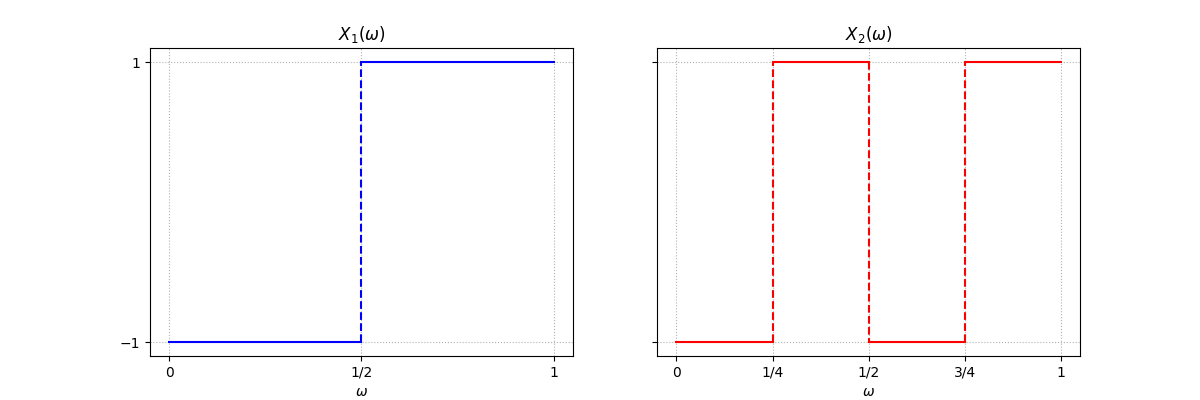
\includegraphics[width=0.8\textwidth]{rademacher_plots.png}
\caption{The first two Rademacher functions.}
\label{fig:rademacher}
\end{figure}% --- CHUNK_METADATA_START ---
% src_checksum: f43f97621087a1ade0cabfff3ef247aa36a0d61778a69e0c21f625fc722cc719
% needs_review: True
% --- CHUNK_METADATA_END ---
To show that $(X_n)_{n \geq 1}$ are independent, it suffices to show that for all $\varepsilon_1, \dots, \varepsilon_n \in \{-1, 1\}$, we have $P(X_1=\varepsilon_1, \dots, X_n=\varepsilon_n) = \prod_{i=1}^n P(X_i=\varepsilon_i)$.% --- CHUNK_METADATA_START ---
% src_checksum: 6d38910023eedf3e9c2c3372dd4ed6dd34ec713a5c79d25ddbabff6debb69ce1
% --- CHUNK_METADATA_END ---
\begin{align*}
    P(X_1=\varepsilon_1, \dots, X_n=\varepsilon_n) &= \lambda(\{\omega \in [0,1[ : \forall i \in \{1..n\}, X_i(\omega)=\varepsilon_i\}) \\
    &= \lambda(\{\omega \in [0,1[ : \forall i \in \{1..n\}, \omega_i = \frac{1+\varepsilon_i}{2}\})
\end{align*}% --- CHUNK_METADATA_START ---
% src_checksum: 0b75d404e16c44d2b357e61e40b8a4cc182ba10ea983d20d05ff003889e25e3e
% needs_review: True
% --- CHUNK_METADATA_END ---
The set of all $\omega$ whose first $n$ binary digits are fixed forms a dyadic interval of length $1/2^n$. For example, if $\varepsilon_1=1, \varepsilon_2=-1$, we look for the $\omega$ with $\omega_1=1, \omega_2=0$, that is, $\omega \in [0.10_2, 0.11_2) = [1/2, 3/4[$. The length is $1/4 = 1/2^2$.
Therefore, $P(X_1=\varepsilon_1, \dots, X_n=\varepsilon_n) = \frac{1}{2^n}$.
Since $P(X_i=\varepsilon_i) = 1/2$ for all $i$, we indeed have $\prod_{i=1}^n P(X_i=\varepsilon_i) = (\frac{1}{2})^n$.
The variables are therefore independent. We have an infinite sequence of independent "coins".% --- CHUNK_METADATA_START ---
% src_checksum: 070062be8edf7cc1b58ac008af2d9da651166b5c74af915364e4ee03c43be65a
% needs_review: True
% --- CHUNK_METADATA_END ---
\section{Random walk on the integers}% --- CHUNK_METADATA_START ---
% src_checksum: 2f9cadafc2d0e545c3008c356c34707bd5c1dc35cabd852033bb6306f4e68b7a
% needs_review: True
% --- CHUNK_METADATA_END ---
We model a symmetric random walk on $\mathbb{Z}$.% --- CHUNK_METADATA_START ---
% src_checksum: 04df92b142d5f30126a85e293b964fc08877d109631f9a72475c6b1268d5495c
% needs_review: True
% --- CHUNK_METADATA_END ---
\begin{itemize}
    \item The walk starts at 0.
    \item At each step, a fair coin is flipped.
    \item Heads: take a step of +1 (to the right). Tails: take a step of -1 (to the left).
    \item The operation is repeated from the new position.
\end{itemize}% --- CHUNK_METADATA_START ---
% src_checksum: 97cd74d1f15e5a01844e1d0f54bb376c7a965a55b452fb4aa1764bcd0f669ae9
% needs_review: True
% --- CHUNK_METADATA_END ---
Let us denote $S_n$ as the position of the walker after $n$ steps. Formally:
\[
S_0 = 0, \quad S_n = X_1 + X_2 + \dots + X_n,
\]
where the $(X_i)$ are a sequence of i.i.d. random variables with $P(X_i=1)=P(X_i=-1)=1/2$.% --- CHUNK_METADATA_START ---
% src_checksum: 2f7faafdd26ec96ecfc13016aae2c0fdfbd9935285a1feefd208567dd058c58f
% needs_review: True
% --- CHUNK_METADATA_END ---
\begin{center}
"Lighter" \quad $\longleftrightarrow$ \quad 0 \quad $\longleftrightarrow$ \quad "Streetlight"
\end{center}% --- CHUNK_METADATA_START ---
% src_checksum: 8564352d7c741e2f9ff543d69df3f946c65291409e3260795c63d7e8d8e257a7
% needs_review: True
% --- CHUNK_METADATA_END ---
A natural question is: what is the probability that the walker will one day pass by its starting point (the "original lamppost") again? We therefore seek to calculate:
\[
P(\exists n \in \mathbb{N}^*, S_n = 0) = P\left(\bigcup_{n=1}^\infty \{S_n=0\}\right).
\]
For $S_n=0$ to occur, there must be as many +1 steps as -1 steps. The total number of steps $n$ must therefore be even. Let us set $n=2k$.
First, we calculate the probability of returning to 0 after $2k$ steps.
Let $\alpha$ be the number of +1 steps and $\beta$ the number of -1 steps. We must have $\alpha+\beta=2k$ and $\alpha-\beta=0$, which implies $\alpha=\beta=k$.
The number of paths of length% --- CHUNK_METADATA_START ---
% src_checksum: 4f7fad2778962a859f07413730675253cc44d6721c21a3067a025be5f50d0b42
% needs_review: True
% --- CHUNK_METADATA_END ---
$2k$ returning to the origin is the number of ways to choose the $k$ steps +1 among the $2k$ steps, which is $\binom{2k}{k}$. The total number of possible paths of length $2k$ is $2^{2k}$.
Thus,
\[
P(S_{2k}=0) = \frac{\binom{2k}{k}}{2^{2k}}.
\]
Using Stirling's approximation, $m! \sim \sqrt{2\pi m} (m/e)^m$, we find:
\[
P(S_{2k}=0) \approx \frac{1}{\sqrt{\pi k}} \quad \text{for } k \to \infty.
\]
The probability of returning to the origin at a given time tends towards 0.% --- CHUNK_METADATA_START ---
% src_checksum: fa3fa9ddb82f7f45be9507ccb3977af64ef2e937e45f408d5a7c22b15169e52f
% needs_review: True
% --- CHUNK_METADATA_END ---
\begin{figure}[H]
\centering
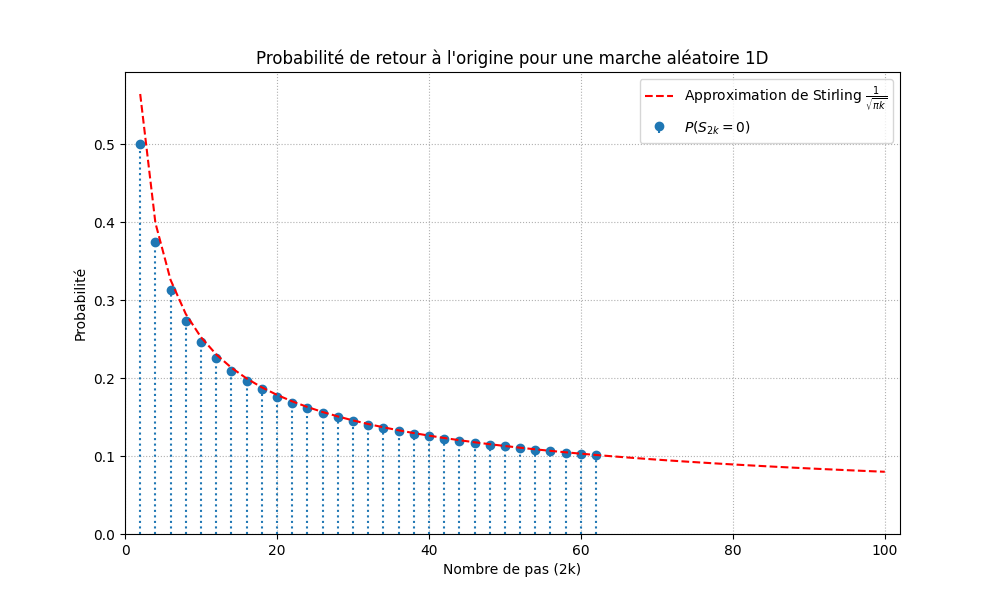
\includegraphics[width=0.8\textwidth]{proba_return_zero.png}
\caption{Evolution of $P(S_{2k}=0)$ as a function of the number of steps.}
\label{fig:return_prob}
\end{figure}% --- CHUNK_METADATA_START ---
% src_checksum: 68860cabcd64ad3b4a7300cb81fd2f5f39fd899ede470c7205bba89ffa76d62a
% needs_review: True
% --- CHUNK_METADATA_END ---
To calculate the probability of returning \emph{one day}, we decompose the event into a union of disjoint events: the first return to the origin. Let $f_{2k} = P(S_2 \neq 0, \dots, S_{2k-2} \neq 0, S_{2k}=0)$.
The probability of returning one day is $\sum_{k=1}^\infty f_{2k}$.% --- CHUNK_METADATA_START ---
% src_checksum: a3dd141905ac0491c67ff87546e2418adc4a4fc7cb8f5b1d2bf5f57a9c062ded
% needs_review: True
% --- CHUNK_METADATA_END ---
\begin{lemma}
The probability of first return at time $2k$ is related to the return probability by the (non-trivial) relation:
\[
f_{2k} = \frac{1}{2k-1} P(S_{2k}=0) \quad (\text{for } k \ge 1).
\]
\end{lemma}% --- CHUNK_METADATA_START ---
% src_checksum: a5d38687044daa576ad57b54a136334f4c7d0013235867472615d7f2a4c28976
% needs_review: True
% --- CHUNK_METADATA_END ---
The probability of returning one day is therefore $\sum_{k=1}^\infty f_{2k}$. It turns out that this sum equals 1.
\[
P(\exists n \in \mathbb{N}^*, S_n = 0) = \sum_{k=1}^\infty f_{2k} = 1.
\]
The simple symmetric random walk on $\mathbb{Z}$ is therefore \emph{recurrent}: it is certain to return to its starting point.
